\documentclass{article}

% Maths
\usepackage{amsmath}

% Hyperlink
\usepackage{hyperref}
\hypersetup{
    colorlinks=true,
    linkcolor=blue,
    filecolor=magenta,      
    urlcolor=cyan,
    pdfpagemode=FullScreen,
}

% Figures
\usepackage{graphics, float, subfig}
\usepackage[pdflatex]{graphicx}

% Itemize
\renewcommand{\labelitemi}{\textbullet}
\renewcommand{\labelitemii}{\textbullet}
\renewcommand{\labelitemiii}{\textbullet}

% Margins
\usepackage[margin=1in]{geometry}

% Helpful commands
\newcommand{\x}{\mathbf{x}}
\newcommand{\V}{\mathbf{v}} % \v already defined
\newcommand{\y}{\mathbf{y}}
\newcommand{\X}{\mathbf{X}}
\newcommand{\A}{\mathbf{A}}
\newcommand{\B}{\boldsymbol\beta} % \b already defined
\newcommand{\I}{\mathbf{I}}
\newcommand{\D}{\mathbf{D}}

\begin{document}
 
% TODO: Make a nice title page
APPM 4600 Project 3: Regularization in Least Squares\\
Alexey Yermakov, Logan Barnhart, and Tyler Jensen

\section{Introduction}
\subsection{Project Summary}

%TODO: Complete when we've finished the project
This project explores data fitting. In particular, we explore fitting polynomials of various degrees to noisy data. The system of equations that we're solving to obtain the coefficients of our polynomial is overdetermined. To this end, we derive the normal equation with an extra regularization term, resulting in what is commonly called the ``Ridge Estimator''. Then, we use this derivation to do some data fitting in software and analyze our results. Motivated by the Ridge Estimator, we generalize this further by deriving the Tikhonov estimator and doing a similar exploration of its effects on data fitting.

\subsection{Assumptions}

This project makes heavy use of linear algebra. As such, the reader should be familiar with common matrix operations, such as: matrix multiplication, matrix addition, matrix subtraction, and what the transpose of a matrix is. Additionally, the reader should be comfortable with the concept of a derivative. Lastly, the reader should understand how a vector and a row/column matrix are related.

\subsection{Background}

One idea that is used heavily in this project is the norm of a vector. A vector norm is a way of quantifying the ``size'' or ``distance'' of a vector from the origin. The notation for a norm is $||\cdot||$, where $\cdot$ is replaced with the vector we're taking the norm of. We'll now introduce two norms used in this project:

\begin{itemize}
    \item The 1-Norm, which is denoted by $||\cdot||_1$. Given a vector $\V=\{v_0,v_1,...,v_n\}$, $||\V||_1=\sum_{n=0}^{n}|v_i|$, which is the sum of the absolute value of each element in the vector.
    \item The 2-Norm, which is denoted by $||\cdot||_2$. Given a vector $\V=\{v_0,v_1,...,v_n\}$, $||\V||_2=\left(\sum_{n=0}^{n}|v_i|^2\right)^{\frac{1}{2}}$, which is the square root of sum of the squares of the absolute value of each element in the vector. In fact, it is common to see $||\V||_2^{2}=\sum_{n=0}^{n}(|v_i|^2)$, which gets rid of the square root.
\end{itemize}

Now we can introduce the core exploration of this project: data fitting and regularization. Data fitting is the process of fitting a function to a set of collected data. In this project, the ``fitting'' is done by finding the coefficients of the sum of a set of basis functions. The basis functions we use in this project are $\{1,x,x^2,...,x^m\}$, where $m$ is chosen differently depending on the degree of the polynomial we're fitting to the data. This fitted polynomial is called our approximation. So, given collected data like $\{x_i,y_i\}$ ($0 \le i \le n$) we try to fit a polynomial of degree $m$ ($p_m(x)=\beta_0+\beta_1*x+\ldots+\beta_m*x^m$) to the collected data. (Note: we require $m<n$ to have an overdetermined system, more on this later). How does this process work? We need to define a metric describing how ``close'' our approximation is to the data. One simple metric is that at each data point $\{x_i,y_i\}$, our approximation is off by the difference in $y$-values: $|p_m(x_i)-y_i|$. However, this metric needs to somehow be combined to give us a single scalar value for our choice of coefficients $\{\beta_0,\beta_1,...,\beta_m\}$ across the entire collection of data points. We can use our previously introduced idea of a norm to assist us with this. We can create a vector $\V$ where the $i$-th element is equal to $v_i=|p_m(x_i)-y_i|$. Then, we can pass this vector into a norm $||\cdot||$ to get a single scalar which tells us how ``far'' off our approximation polynomial is from fitting to the given data.

This exact idea is used to derive the normal equation. Note that $p_m(x_i)=\beta_0+\beta_1*x_i+\ldots+\beta_m*x_i^m$. Using this as motivation, we can define the following matrices:

\begin{equation*}
    \X =
    \begin{bmatrix}
        1 & x_0 & x_0 ^2 & \ldots & x_0^m \\
        1 & x_1 & x_1 ^2 & \ldots & x_1^m \\
        1 & x_2 & x_2 ^2 & \ldots & x_2^m \\
        \vdots & \vdots & \vdots & \ddots & \vdots \\
        1 & x_n & x_n ^n & \ldots & x_n^m \\
    \end{bmatrix}
    \quad
    \B =
    \begin{bmatrix}
        \beta_0\\
        \beta_1\\
        \vdots\\
        \beta_m
    \end{bmatrix}
    \quad
    \y =
    \begin{bmatrix}
        y_0\\
        y_1\\
        \vdots\\
        y_n
    \end{bmatrix}
\end{equation*}

Where $dim(\X)=(n+1)\times(m+1)$, $dim(\B)=(m+1)\times(1)$, and $dim(\y)=(n+1)\times(1)$.

So, we can get something similar to our vector $\V$ by $\X\B-\y$:

\begin{equation*}
    \X\B-\y = 
    \begin{bmatrix}
        p_m(x_0) - y_0 \\ 
        p_m(x_1) - y_1 \\ 
        p_m(x_2) - y_2 \\ 
        \vdots \\ 
        p_m(x_n) - y_n \\ 
    \end{bmatrix}
    =
    \begin{bmatrix}
        \beta_0 + \beta_1*x_0 + \beta_2*x_0 ^2 + \ldots + \beta_m*x_0^m - y_0\\
        \beta_0 + \beta_1*x_1 + \beta_2*x_1 ^2 + \ldots + \beta_m*x_1^m - y_1\\
        \beta_0 + \beta_1*x_2 + \beta_2*x_2 ^2 + \ldots + \beta_m*x_2^m - y_2\\
        \vdots  \\
        \beta_0 + \beta_1*x_n + \beta_2*x_n ^n + \ldots + \beta_m*x_n^m - y_n\\
    \end{bmatrix}
\end{equation*}

To get the absolute value for each term as we had before, we can pass $\X\B-\y$ into the 1-Norm! Thus, $||\V||_1=||\X\B-\y||_1$ is exactly what we had earlier with $|p_m(x_i)-y_i|$! Note, however, that this time the absolute values come from the 1-Norm and not how we're defining the vector $\V$. The next step is to find the $\B$ such that $||\X\B-\y||_1$ is minimized, giving us the formula: $\arg \min_{\B} ||\X\B-\y||_{1}$. The solution to this formula then gives us the coefficients to $p_m(x)$ that fit the polynomial to the data! Note that depending on the formula we're minimizing, our polynomial fit may be different. Traditionally, the 2-Norm is used: $\arg \min_{\B} ||\X\B-\y||_{2}$. As mentioned earlier, we want $m<n$ so that we have more equations than variables we're solving for (that is, we have more data points $\{x_i, y_i\}$ than coefficients $\beta_i$). This leads to a closed form solution to the equation $\arg \min_{\B} ||\X\B-\y||_{2}$: $\B = (\X^T\X)^{-1}\X^T \y$ (the derivation for this is below, since it's a special case of the Ridge Estimator with $\lambda=0$). In fact, this method in general is called Least-Squares.

What does this look like in practice? Below is a graph visualizing noisy data generated by a line with the original function. 

\begin{figure}[H]
    \centering
    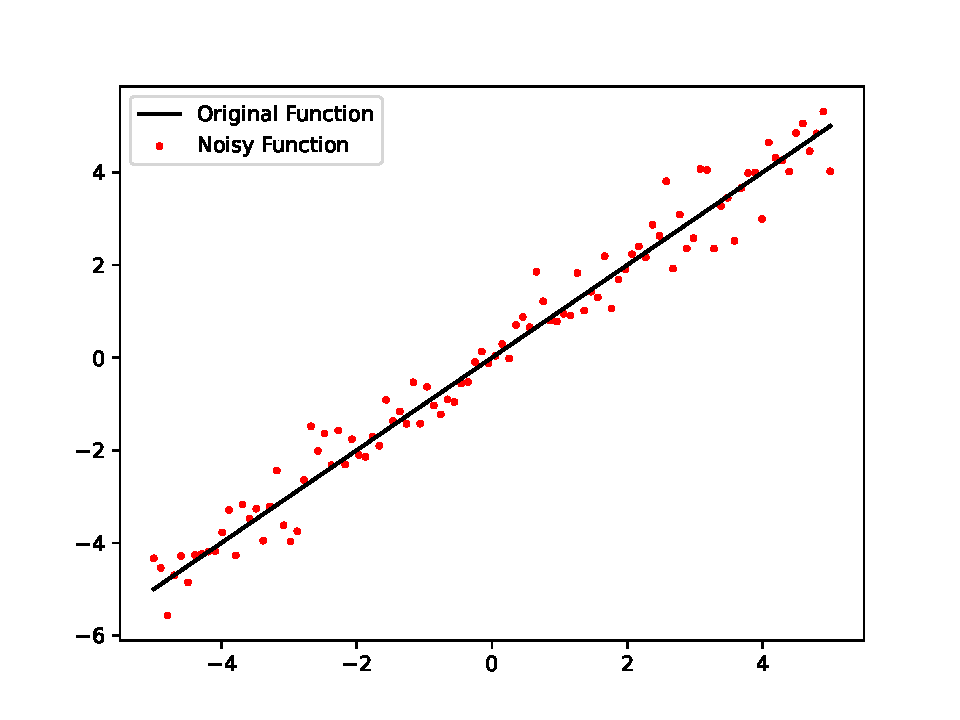
\includegraphics[width=12cm]{../Images/intro_1.pdf}
    \caption{Line with a noisy version of the line.}
\end{figure}

Suppose we didn't know what the original function looked like. We would have to use data fitting to find the coefficients of a degree one polynomial to the data. However, this assumes we know the degree of the function that generated the noisy function. Often times, we don't know the underlying function. This could lead to the following situation, where it appears our noisy data is quadratic when the true function is cubic.

\begin{figure}[H]
    \centering
    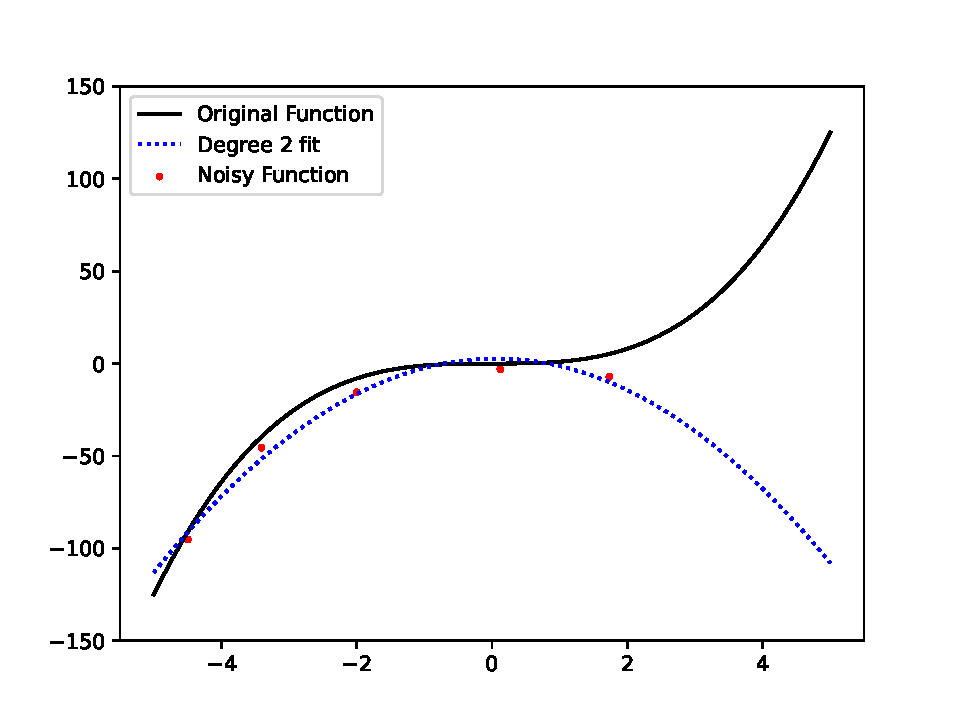
\includegraphics[width=12cm]{../Images/intro_2.pdf}
    \caption{Cubic with a noisy version of the cubic. Further, there is a hypothetical data-fitted quadratic in blue.}
\end{figure}

Here, we because we don't have enough data, it appears that a quadratic is best for approximating the noisy data, but the true function is in fact cubic. There may also be situations where the true function is not a polynomial, so the basis functions we are using in this project will never result in the underlying function. Additionally, it is possible to overfit to the data by having an approximate polynomial with degree larger than the underlying function, resulting in the following situation, called data overfitting:

\begin{figure}[H]
    \centering
    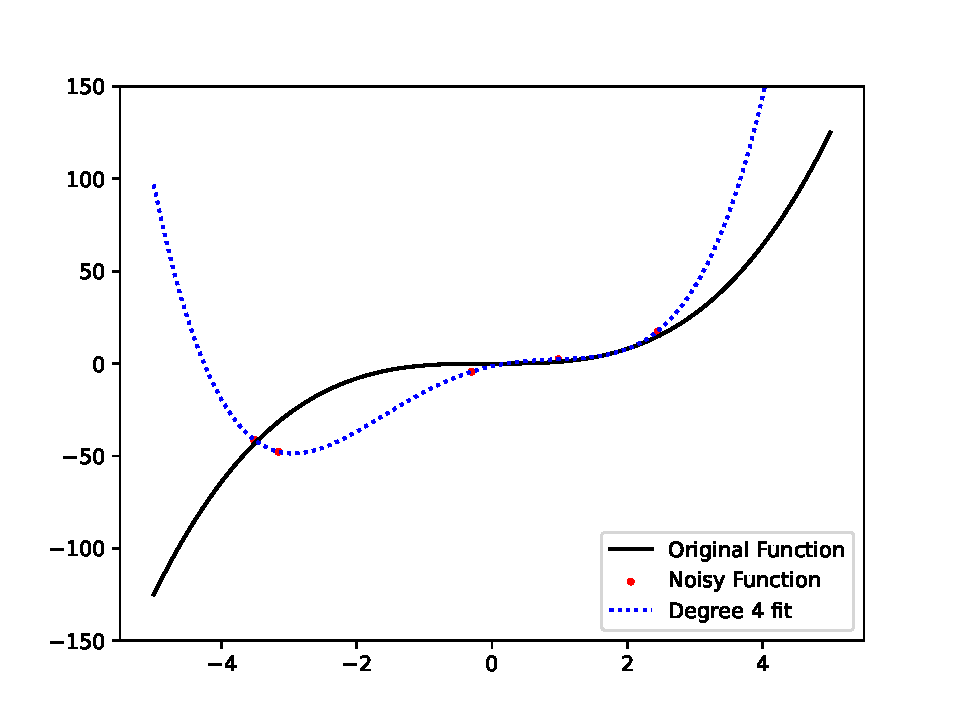
\includegraphics[width=12cm]{../Images/intro_3.pdf}
    \caption{An example of overfitting to data. A fourth-degree polynomial is fit to data generated by a third-degree polynomial.}
\end{figure}

Given that there are lots of different considerations when fitting data, in this project we explore regularization, which aims to reduce the effects of the latter figure above. As such, we want our approximate polynomial to be a good fit for data generated by a polynomial of lower degree. This situation occurs naturally since in practice we often don't know the underlying function that we're approximating. One way to add regularization is by penalizing the relative size of the coefficients for our approximate polynomial: $\gamma||\B||_{2}^{2}$. This is an extension to Least Squares called Ridge Regression! We can now go on to the contents of the project, where we first derive the Ridge Estimator.

\section{Ridge Regression}
\subsection{Deriving the Ridge Estimator}

The equation for regularized least squares is:

\begin{equation} \label{eqn:rls}
    \arg \min_{\B} ||\X\B-\y||_{2}^{2} + \gamma||\B||_{2}^{2}
\end{equation}

Recalling that $||\B||_{2}^{2}=\B^T \B$, we'll rewrite $||\X\B-\y||_{2}^{2} + \gamma||\B||_{2}^{2}$:

\begin{equation*}
\begin{split}
    & ||\X\B-\y||_{2}^{2} + \gamma||\B||_{2}^{2} =\\
    & =  (\X\B - \y)^T (\X\B - \y) + \gamma \B^T \B \\ 
    & =  ((\X\B)^T - \y^T) (\X\B - \y) + \gamma \B^T \B \\ 
    & =  (\B^T\X^T - \y^T) (\X\B - \y) + \gamma \B^T \B \\ 
    & = \B^T \X^T \X\B - \B^T \X^T \y - \y^T \X\B + \y^T \y + \gamma \B^T \B
\end{split}
\end{equation*}

Before we proceed further, we'll define what $\X$, $\y$, and $\B$ are. We want a least-squares fit to an $m$-degree polynomial $p_m(x)=\beta_0+\beta_1*x+\ldots+\beta_m*x^m$ where we have $n$ data points $\{x_i,y_i\}$. To have our system be overdetermined, we also assume $n > m$.

\begin{equation*}
    \X =
    \begin{bmatrix}
        1 & x_0 & x_0 ^2 & \ldots & x_0^m \\
        1 & x_1 & x_1 ^2 & \ldots & x_1^m \\
        1 & x_2 & x_2 ^2 & \ldots & x_2^m \\
        \vdots & \vdots & \vdots & \ddots & \vdots \\
        1 & x_n & x_n ^n & \ldots & x_n^m \\
    \end{bmatrix}
    \quad
    \B =
    \begin{bmatrix}
        \beta_0\\
        \beta_1\\
        \vdots\\
        \beta_m
    \end{bmatrix}
    \quad
    \y =
    \begin{bmatrix}
        y_0\\
        y_1\\
        \vdots\\
        y_n
    \end{bmatrix}
\end{equation*}

Where $dim(\X)=(n+1)\times(m+1)$, $dim(\B)=(m+1)\times(1)$, and $dim(\y)=(n+1)\times(1)$.

$ $ %Newline

We'll now prove $\B^T\X^T\y = \y^T\X\B$. Note first that $(\y^T\X\B)^T=\B^T\X^T\y$. Further, $dim(\B^T\X^T\y) = (1) \times (1) = dim(\y^T\X\B)$. Also, note that the transpose of a $1 \times 1$ matrix is the same matrix: $[c]^T=[c]$. It then follows that $\B^T\X^T\y = \y^T\X\B$, completing the proof.

$ $ %Newline

So,

\begin{equation} \label{eqn:rls_prod}
\begin{split}
    &\B^T \X^T \X\B - \B^T \X^T \y - \y^T \X\B + \y^T \y + \gamma \B^T \B = \\ 
    & = \B^T \X^T \X\B -2 \y^T \X\B + \y^T \y + \gamma \B^T \B\\
    & = (\X\B)^T(\X\B) -2 \y^T \X\B + \y^T \y + \gamma \B^T \B
\end{split}
\end{equation}

Now, we'll show what each of the above values (since each matrix is $1 \times 1$, meaning it's a scalar) actually is:

\begin{equation} \label{eqn:Ax}
\begin{split}
    & \X\B = \\
    & =
    \begin{bmatrix}
        1 & x_0 & x_0 ^2 & \ldots & x_0^m \\
        1 & x_1 & x_1 ^2 & \ldots & x_1^m \\
        1 & x_2 & x_2 ^2 & \ldots & x_2^m \\
        \vdots & \vdots & \vdots & \ddots & \vdots \\
        1 & x_n & x_n ^n & \ldots & x_n^m \\
    \end{bmatrix}
    \times
    \begin{bmatrix}
        \beta_0\\
        \beta_1\\
        \vdots\\
        \beta_m
    \end{bmatrix}\\
    & =
    \begin{bmatrix}
        \beta_0 + \beta_1 x_0 + \beta_2 x_0 ^2 + \ldots + \beta_m x_0^m \\
        \beta_0 + \beta_1 x_1 + \beta_2 x_1 ^2 + \ldots + \beta_m x_1^m \\
        \beta_0 + \beta_1 x_2 + \beta_2 x_2 ^2 + \ldots + \beta_m x_2^m \\
        \vdots \\
        \beta_0 + \beta_1 x_n + \beta_2 x_n ^2 + \ldots + \beta_m x_n^m \\
    \end{bmatrix}
\end{split}
\end{equation}

Then, $(\X\B)^T \X\B$ is just a simple inner product (we will use the result from \ref{eqn:Ax}):

\begin{equation} \label{eqn:axtax}
\begin{split}
    & (\X\B)^T \X\B = \\
    & =
    \begin{bmatrix}
        \beta_0 + \beta_1 x_0 + \beta_2 x_0 ^2 + \ldots + \beta_m x_0^m \\
        \beta_0 + \beta_1 x_1 + \beta_2 x_1 ^2 + \ldots + \beta_m x_1^m \\
        \beta_0 + \beta_1 x_2 + \beta_2 x_2 ^2 + \ldots + \beta_m x_2^m \\
        \vdots \\
        \beta_0 + \beta_1 x_n + \beta_2 x_n ^2 + \ldots + \beta_m x_n^m \\
    \end{bmatrix} ^T
    \times
    \begin{bmatrix}
        \beta_0 + \beta_1 x_0 + \beta_2 x_0 ^2 + \ldots + \beta_m x_0^m \\
        \beta_0 + \beta_1 x_1 + \beta_2 x_1 ^2 + \ldots + \beta_m x_1^m \\
        \beta_0 + \beta_1 x_2 + \beta_2 x_2 ^2 + \ldots + \beta_m x_2^m \\
        \vdots \\
        \beta_0 + \beta_1 x_n + \beta_2 x_n ^2 + \ldots + \beta_m x_n^m \\
    \end{bmatrix} \\
    & = (\beta_0 + \beta_1 x_0 + \ldots + \beta_m x_0^m)^ 2 + (\beta_0 + \beta_1 x_1 + \ldots + \beta_m x_1^m)^ 2\\
    & + \ldots + (\beta_0 + \beta_1 x_n + \ldots + \beta_m x_n^m)^ 2
\end{split}
\end{equation}

\begin{equation} \label{eqn:2bax}
\begin{split}
    & 2 \y ^T \X \B = \\
    & = 2 \times
    \begin{bmatrix}
        y_0 &
        y_1 &
        \ldots & 
        y_n
    \end{bmatrix}
    \times
    \begin{bmatrix}
        1 & x_0 & x_0 ^2 & \ldots & x_0^m \\
        1 & x_1 & x_1 ^2 & \ldots & x_1^m \\
        1 & x_2 & x_2 ^2 & \ldots & x_2^m \\
        \vdots & \vdots & \vdots & \ddots & \vdots \\
        1 & x_n & x_n ^2 & \ldots & x_n^m \\
    \end{bmatrix}
    \times
    \begin{bmatrix}
        \beta_0\\
        \beta_1\\
        \vdots\\
        \beta_m
    \end{bmatrix}\\
    & = 2 \times
    \begin{bmatrix}
        y_0 + y_1 + y_2 + \ldots + y_n \\
        y_0 x_0 + y_1 x_1 + y_2 x_2 + \ldots + y_n x_n \\
        y_0 x_0^2 + y_1 x_1^2 + y_2 x_2^2 + \ldots + y_n x_n^2 \\
        \vdots\\
        y_0 x_0^m + y_1 x_1^m + y_2 x_2^m + \ldots + y_n x_n^m \\
    \end{bmatrix} ^T
    \times
    \begin{bmatrix}
        \beta_0\\
        \beta_1\\
        \vdots\\
        \beta_m
    \end{bmatrix}\\
    & = 2(\beta_0 (y_0 + y_1 + \ldots + y_n) + \beta_1 (y_0 x_0 + y_1 x_1 + \ldots + y_n x_n) + \ldots + \beta_m (y_0 x_0^m + y_1 x_1^m + \ldots + y_n x_n^m))
\end{split}
\end{equation}

\begin{equation} \label{eqn:gxx}
\begin{split}
    & \gamma \B ^T \B = \\
    & \text{This is a simple inner product multiplied by a scalar} \\
    & = \gamma \beta_0 ^2 + \gamma \beta_1 ^2 + \ldots + \gamma \beta_m^2
\end{split}
\end{equation}

Great! Now lets take the derivates of \ref{eqn:axtax}, \ref{eqn:2bax}, and \ref{eqn:gxx} with respect to $\B$ to get the derivative of \ref{eqn:rls} with respect to $\B$. In effect, we'll get a vector where the $i$-th element is the derivative of \ref{eqn:rls} with respect to $\beta_i$.

First, let's take the derivatives of \ref{eqn:axtax}:

\begin{equation}
\begin{split}
    & \frac{d}{d\B} (\X\B)^T \X\B = \\
    & =
    \begin{bmatrix}
        \frac{d}{d \beta_0} (\X\B)^T \X\B \\
        \frac{d}{d \beta_1} (\X\B)^T \X\B \\
        \vdots \\
        \frac{d}{d \beta_m} (\X\B)^T \X\B \\
    \end{bmatrix}\\
    & =
    \begin{bmatrix}
        2(\beta_0 + \beta_1 x_0 + \dots + \beta_m x_0 ^ m) + 2(\beta_0 + \beta_1 x_1 + \dots + \beta_m x_1 ^ m) + \ldots + 2(\beta_0 + \beta_1 x_n + \dots + \beta_m x_n ^ m)\\
        2 x_0(\beta_0 + \beta_1 x_0 + \dots + \beta_m x_0 ^ m) + 2 x_1(\beta_0 + \beta_1 x_1 + \dots + \beta_m x_1 ^ m) + \ldots + 2 x_n(\beta_0 + \beta_1 x_n + \dots + \beta_m x_n ^ m)\\
        \vdots \\
        2 x_0^m(\beta_0 + \beta_1 x_0 + \dots + \beta_m x_0 ^ m) + 2 x_1^m(\beta_0 + \beta_1 x_1 + \dots + \beta_m x_1 ^ m) + \ldots + 2 x_n^m(\beta_0 + \beta_1 x_n + \dots + \beta_m x_n ^ m)
    \end{bmatrix}\\
    & = 2 \times
    \begin{bmatrix}
        \beta_0 \sum_{i=0}^{n} 1 + \beta_1 \sum_{i=0}^{n} x_i + \beta_2 \sum_{i=0}^{n} x_i^2 + \ldots + \beta_m \sum_{i=0}^{n} x_i ^ m\\
        \beta_0 \sum_{i=0}^{n} x_i + \beta_1 \sum_{i=0}^{n} x_i^2 + \beta_2 \sum_{i=0}^{n} x_i^3 + \ldots + \beta_m \sum_{i=0}^{n} x_i ^ {m+1}\\
        \vdots \\
        \beta_0 \sum_{i=0}^{n} x_i^m + \beta_1 \sum_{i=0}^{n} x_i^{m+1} + \beta_2 \sum_{i=0}^{n} x_i^{m+2} + \ldots + \beta_m \sum_{i=0}^{n} x_i ^ {2m}\\
    \end{bmatrix}\\
    & = 2 \times
    \begin{bmatrix}
        \sum_{i=0}^{n} 1 & \sum_{i=0}^{n} x_i & \sum_{i=0}^{n} x_i ^2 & \ldots & \sum_{i=0}^{n} x_i ^m\\
        \sum_{i=0}^{n} x_i & \sum_{i=0}^{n} x_i ^2 & \sum_{i=0}^{n} x_i ^3 & \ldots & \sum_{i=0}^{n} x_i ^{m+1}\\
        \sum_{i=0}^{n} x_i ^2 & \sum_{i=0}^{n} x_i ^3 & \sum_{i=0}^{n} x_i ^4 & \ldots & \sum_{i=0}^{n} x_i ^{m+2}\\
        \vdots & \vdots & \vdots & \ddots & \vdots \\
        \sum_{i=0}^{n} x_i ^{m} & \sum_{i=0}^{n} x_i ^{m+1} & \sum_{i=0}^{n} x_i ^{m+2} & \ldots & \sum_{i=0}^{n} x_i ^{2m}
    \end{bmatrix}
    \times
    \begin{bmatrix}
        \beta_0 \\
        \beta_1 \\
        \beta_2 \\
        \vdots \\
        \beta_m
    \end{bmatrix}\\
    & = 2 \times
    \begin{bmatrix}
        1 & 1 & 1 & \ldots & 1 \\
        x_0 & x_1 & x_2 & \ldots & x_n \\
        x_0^2 & x_1^2 & x_2 ^2 & \ldots & x_n^2 \\
        \vdots & \vdots & \vdots & \ddots & \vdots \\
        x_0^m & x_1^m & x_2 ^m & \ldots & x_n^m \\
    \end{bmatrix}
    \times
    \begin{bmatrix}
        1 & x_0 & x_0 ^2 & \ldots & x_0^m \\
        1 & x_1 & x_1 ^2 & \ldots & x_1^m \\
        1 & x_2 & x_2 ^2 & \ldots & x_2^m \\
        \vdots & \vdots & \vdots & \ddots & \vdots \\
        1 & x_n & x_n ^2 & \ldots & x_n^m \\
    \end{bmatrix}
    \times
    \begin{bmatrix}
        \beta_0 \\
        \beta_1 \\
        \beta_2 \\
        \vdots \\
        \beta_m
    \end{bmatrix}\\
    &= 2\X ^T \X \B
\end{split}
\end{equation}

Secondly, let's take the derivatives of \ref{eqn:2bax}:

\begin{equation}
\begin{split}
    & \frac{d}{d\B} 2 \y ^T \X \B = \\
    & =
    \begin{bmatrix}
        \frac{d}{d a_0} 2 \y ^T \X \B \\
        \frac{d}{d a_1} 2 \y ^T \X \B \\
        \vdots \\
        \frac{d}{d a_m} 2 \y ^T \X \B \\
    \end{bmatrix}\\
    & = 2 \times
    \begin{bmatrix}
        y_0 + y_1 + \ldots + y_n \\
        y_0x_0 + y_1x_1 + \ldots + y_nx_n \\
        y_0x_0^2 + y_1x_1^2 + \ldots + y_nx_n^2 \\
        \vdots \\
        y_0x_0^m + y_1x_1^m + \ldots + y_nx_n^m \\
    \end{bmatrix}\\
    &= 2 \times
    \begin{bmatrix}
        1 & 1 & 1 & \ldots & 1 \\
        x_0 & x_1 & x_2 & \ldots & x_n \\
        x_0^2 & x_1^2 & x_2 ^2 & \ldots & x_n^2 \\
        \vdots & \vdots & \vdots & \ddots & \vdots \\
        x_0^m & x_1^m & x_2 ^m & \ldots & x_n^m
    \end{bmatrix}
    \times
    \begin{bmatrix}
        y_0\\
        y_1\\
        \vdots\\
        y_n
    \end{bmatrix}\\
    &= 2 \X ^T \y
\end{split}
\end{equation}

Lastly, let's take the derivatives of \ref{eqn:gxx}:

\begin{equation}
\begin{split}
    & \frac{d}{d\B} \gamma \B^T \B = \\
    & =
    \begin{bmatrix}
        \frac{d}{d \beta_0} \gamma \B^T \B \\
        \frac{d}{d \beta_1} \gamma \B^T \B \\
        \vdots \\
        \frac{d}{d \beta_m} \gamma \B^T \B \\
    \end{bmatrix}\\
    &= \gamma \times
    \begin{bmatrix}
        2 \beta_0 \\
        2 \beta_1 \\
        2 \beta_2 \\
        \vdots \\
        2 \beta_m
    \end{bmatrix}\\
    &= 2 \times \gamma \times
    \begin{bmatrix}
        1 & 0 & 0 & \ldots & 0\\
        0 & 1 & 0 & \ldots & 0\\
        0 & 0 & 1 & \ldots & 0\\
        \vdots & \vdots & \vdots & \ddots & \vdots \\
        0 & 0 & 0 & \ldots & 1\\
    \end{bmatrix}
    \times
    \begin{bmatrix}
        \beta_0 \\
        \beta_1 \\
        \beta_2 \\
        \vdots \\
        \beta_m
    \end{bmatrix}\\
    &= 2 \gamma \I \B
\end{split}
\end{equation}

Now we can recall \ref{eqn:rls_prod} and note that to find the minimum of the least squares equation given by \ref{eqn:rls} we can find where the derivative of \ref{eqn:rls_prod} is equal to zero:

\begin{equation}
\begin{split}
    \frac{d}{d \B} (\frac{}{}(\X\B)^T(\X\B) -2 \y^T \X\B + \y^T \y + \gamma \B^T \B) &= 0 \\
    2 \X ^T \X \B - 2 \X ^T \y + 2 \gamma \I \B &= 0 \\
    \X ^T \X \B - \X ^T \y + \gamma \I \B &= 0 \\
    \X ^T \X \B + \gamma \I \B - \X ^T \y &= 0 \\
    ( \X ^T \X + \gamma \I ) \B - \X ^T \y &= 0 \\
    ( \X ^T \X + \gamma \I ) \B  &= \X ^T \y \\
    \B &= ( \X ^T \X + \gamma \I )^{-1} \X ^T \y  \\
\end{split}
\end{equation}

We have now arrived at the equation for Ridge Regression! We note that there is a typo in the project description for the equation $E_{ridge}=( \X ^T \X + \gamma \I )^{-1} \X ^T$, where there is no trailing $\y$.

\section{Tikhonov Regression}
We can further generalize the loss function used for Ridge Regression if we notice that:


\begin{align*}
\arg \min_{x} ||\X\B-\y||_{2}^{2} + \gamma||\B||_{2}^{2} \\
\end{align*}


is equivalent to 


\begin{align*}
\arg \min_{x} ||\X\B-\y||_{2}^{2} + ||\sigma \I \B||_{2}^{2} \\
\end{align*}

where $\sigma = \sqrt{\gamma}$. We can generalize this by replacing $\sigma \I $ with various other \emph{weight matrices} to 'focus' the penalization on certain qualities or terms of $\B$. 

For example, we can use forward differences to estimate the derivative of a vector by using the matrix:

\begin{align*}
  \D = \begin{bmatrix}
    -\frac{1}{2} & 0 & \frac{1}{2} & 0 & \dots & 0 \\
    0 & -\frac{1}{2} & 0 & \frac{1}{2} & 0 & \vdots \\
    \vdots & 0 & \ddots & \ddots & \ddots & 0 \\
    0 & \dots & 0 & -\frac{1}{2} & 0 & \frac{1}{2} \\ 
  \end{bmatrix}\\
\end{align*}

Note that $\D$ is $(n-2) \times n $. If we put this in our loss function, it becomes: 

\begin{align*}
\arg \min_{x} ||\X\B-\y||_{2}^{2} + \lambda^2||\D \B||_{2}^{2} \\
\end{align*}

Where $\lambda$ is just a general weighting constant to control how much we want to penalize that last term. Now instead of just penalizing the magnitude of $\B$, we are penalizing its derivative - or in other words, forcing the resulting polynomial to be smooth. This will obviously change the solution of our estimator to solve the above loss function. 

\subsection{Exploring the Ridge Estimator}

With our derivation of the Ridge Estimator, we can now implement and test the Ridge Estimator on some data.
All code is in python 3, any random data was generated by using numpy's random number generator with seed 50. We will now construct
some data that we will test our Ridge Estimator implementation on. We take 20 random samples from the line $y = 3x + 2$ with Gaussian noise from a standard
normal distribtution. We now randomly sample 10 of these data points and will use them to fit/train our ridge regression model on, we will refer to these points as our 
training data, and the remaining 10 points we will call our validation data and will be used to measure the accuracy of our model using Residual Sum of Squares (also known as Sum of Squared Errors)

For this data we will try to find the line of best fit, that is find $m$ and $c$ in $y = mx + b$. We begin by trying $\gamma = 0$. This case reduces ridge regression to 
just normal linear regression/ordinary least squares. We also try $\gamma = 0.1$, this is the first real test of ridge regression. RSS compared below

From this we see that we achieved a lower RSS with $\gamma = 0.1$. That means that we have already improved over ordinary least squares! Ridge Regression has already shown to be an improvement. 
But we just tried some random $\gamma$ value, are there other values of $\gamma$ where the performance is even better? There's no analytic way to test this,
so we try a whole lot of $\gamma$'s and see what happens.


From this graph we see that our lowest RSS's occur for $\gamma$'s from $[0,10]$. We now try those $\gamma$'s. 

We achieve a min RSS of at $\gamma = 1$. Thus ridge regression gives us a model that performs about % 
better than what we had with ordinary least square. That's quite an exciting result. Let's see if this translates to other functions/models.


We now consider $y = x^2$. We begin by taking 20 random samples from the interval $[-5,5]$ and then splitting the data into our training data and validation
data as we did for $y = 3x + 2$. 

Now we want to try and fit our data to the model $y = $. We try a similar approach as we did before, testing 
\subsection{Deriving the Tikhonov Estimator}

As we saw when deriving the ridge estimator, to find this estimator we want to solve

\begin{align*}
\frac{d}{d\B} \left[ ||\X\B-\y||_{2}^{2} + \lambda^2||\D \B||_{2}^{2} \right] = 0 \\
\end{align*}
or, if we expand that similar to the loss function for ridge estimation, 

\begin{align*}
\frac{d}{d\B} \left[ (\X\B)^T(\X\B) -2 \y^T \X\B + \y^T \y + \lambda^2(\D\B)^{\textrm{T}}(\D\B) \right] = 0 \\
\end{align*}

From the ridge estimator derivation we already know that 
\begin{align*}
\frac{d}{d\B} [ (\X\B)^{\textrm{T}} \X\B ] = 2\X^{\textrm{T}}\X\B \\
\frac{d}{d\B} [ (2\y^{\textrm{T}} \X\B ] = 2\X^{\textrm{T}}\y
\end{align*}

So what is $\frac{d}{d\B} [ (\D\B)^{\textrm{T}}\D\B ] $? Well, 

\begin{align*}
  \D\B &= \begin{bmatrix}
    -\frac{1}{2} & 0 & \frac{1}{2} & 0 & \dots & 0 \\
    0 & -\frac{1}{2} & 0 & \frac{1}{2} & 0 & \vdots \\
    \vdots & 0 & \ddots & \ddots & \ddots & 0 \\
    0 & \dots & 0 & -\frac{1}{2} & 0 & \frac{1}{2} \\ 
  \end{bmatrix} 
  \begin{bmatrix}
  \beta_0 \\
  \beta_1 \\
  \vdots \\
  \beta_n
  \end{bmatrix} \\\\
  &= \frac{1}{2}\begin{bmatrix}
  \beta_2 - \beta_0 \\ 
  \beta_3 - \beta_1 \\ 
  \beta_4 - \beta_2 \\
  \vdots \\
  \beta_n - \beta_{n-2}
  \end{bmatrix}
\end{align*}

So it follows that

\begin{align*}
  &(\D\B)^{\textrm{T}}(\D\B) = 
  \begin{bmatrix}
  \frac{\beta_2 - \beta_0}{2} \\ 
  \frac{\beta_3 - \beta_1}{2} \\ 
  \frac{\beta_4 - \beta_2}{2} \\
  \vdots \\
  \frac{\beta_n - \beta_{n-2}}{2}
  \end{bmatrix} ^ {\textrm{T}}
   \begin{bmatrix}
  \frac{\beta_2 - \beta_0}{2} \\ 
  \frac{\beta_3 - \beta_1}{2} \\ 
  \frac{\beta_4 - \beta_2}{2} \\
  \vdots \\
  \frac{\beta_n - \beta_{n-2}}{2}
  \end{bmatrix} \\\\
  &= \left( \frac{(\beta_2 - \beta_0)^2}{4} + \frac{(\beta_3 - \beta_1)^2}{4} + \dots \frac{(\beta_n - \beta_{n-2})^2}{4} \right)
\end{align*}

Then it follows that 

\begin{align*}
\frac{d}{d\B} \left[ (\D\B)^{\textrm{T}}(\D\B) \right] = 
\begin{bmatrix}
- \frac{\beta_2 - \beta_0}{2} \\\\
- \frac{\beta_3 - \beta_2}{2} \\\\
\frac{\beta_2 - \beta_0}{2} - \frac{\beta_4 - \beta_2}{2}\\
\vdots \\
\frac{\beta_{n-2} - \beta_{n-4}}{2} - \frac{\beta_n - \beta_{n-2}}{2}\\\\
\frac{\beta_{n-1} - \beta_{n-3}}{2} \\\\
\frac{\beta_n - \beta_n-2}{2}
\end{bmatrix}
\end{align*}

This initially doesn't seem like anything useful, but note that

\begin{align*}
\D^{\textrm{T}}\D\B &= 
\begin{bmatrix}
  -\frac{1}{2} & 0  & 0 & \dots & 0\\
  0 & -\frac{1}{2} & 0  & \dots & 0 \\
  \frac{1}{2} & 0 & \ddots   & \dots & 0 \\
  0 & \frac{1}{2} & 0  & -\frac{1}{2}  & 0\\
  \vdots & 0 & \ddots & 0& -\frac{1}{2} \\
  0 & \dots & 0 & \frac{1}{2} & 0 \\
  0 & \dots & 0 & 0 & \frac{1}{2}
\end{bmatrix}
\begin{bmatrix}
\frac{\beta_2 - \beta_0}{2} \\
\frac{\beta_3 - \beta_1}{2} \\
\vdots \\
\frac{\beta_n - \beta_{n-2}}{2} \\
\end{bmatrix} \\ \\
&= 
\begin{bmatrix}
-\frac{\beta_2 - \beta_0}{4} \\\\
-\frac{\beta_3 - \beta_1}{4} \\\\
\frac{\beta_2 - \beta_0}{4} - \frac{\beta_4 - \beta_2}{4} \\\\
\vdots \\
\frac{\beta_{n-2} - \beta_{n-4}}{4} - \frac{\beta_n - \beta_{n-2}}{4}\\\\
\frac{\beta_{n-1} - \beta_{n-3}}{4} \\\\
\frac{\beta_n - \beta_n-2}{4}
\end{bmatrix}
\end{align*}
So, it's true that 
\begin{align*}
\frac{d}{d\B} \left[ (\D\B)^{\textrm{T}}(\D\B) \right] = 2\D^{\textrm{T}}\D\B\\
\end{align*}

Finally we can solve for the $\B$ that satisfies

\begin{align*}
\frac{d}{d\B} \left[||\X\B-\y||_{2}^{2} + \lambda^2||\D \B||_{2}^{2} \right] = 0 \\
\end{align*}
or,
\begin{align*}
 2\X^{\textrm{T}}\X\B - 2\X^{\textrm{T}}\y + 2\lambda^2 \D^{\textrm{T}}\D\B = 0 \\
 \X^{\textrm{T}}\X\B - \X^{\textrm{T}}\y + \lambda^2 \D^{\textrm{T}}\D\B = 0 \\
 \X^{\textrm{T}}\X\B  + \lambda^2 \D^{\textrm{T}}\D\B = \X^{\textrm{T}}\y\\
  (\X^{\textrm{T}}\X  + \lambda^2 \D^{\textrm{T}}\D)\B = \X^{\textrm{T}}\y\\
\end{align*}
Thus
\begin{align*}
\B = (\X^{\textrm{T}}\X  + \lambda^2 \D^{\textrm{T}}\D)^{-1}\X^{\textrm{T}}\y\\
\end{align*}

Generally speaking, a loss function with weight matrix $\mathbf{\Gamma}$ of the form

\begin{align*}
\arg \min_{x}||\X\B-\y||_{2}^{2} + ||\textbf{$\Gamma$} \B||_{2}^{2}
\end{align*}

will be solved by 

\begin{align*}
\B = (\X^{\textrm{T}}\X  + \mathbf{\Gamma}^{\textrm{T}}\mathbf{\Gamma})^{-1}\X^{\textrm{T}}\y\\
\end{align*}

but weight matrices can be customized to such a degree that it's best to verify this property for each case. 

\end{document}